\documentclass[12pt,a4paper,twoside]{article}

\setlength{\oddsidemargin}{-0.4mm} % 25 mm left margin - 1 in
\setlength{\evensidemargin}{\oddsidemargin}
\setlength{\topmargin}{-5.4mm} % 20 mm top margin - 1 in
\setlength{\textwidth}{160mm} % 25 mm right margin
\setlength{\textheight}{247mm} % 20 mm bottom margin
\setlength{\headheight}{5mm}
\setlength{\headsep}{5mm}
\setlength{\parindent}{0mm}
\setlength{\parskip}{\medskipamount}
\usepackage{graphicx}
\newcommand{\subsubsubsection}[1]{\vspace{0.01in}\textbf{#1}\vspace{0.01in}\\}
\usepackage{float}
\usepackage{array}
\raggedbottom


\begin{document}

\begin{titlepage}
\begin{center}

\textsc{\LARGE University of Cambridge}\\[3.5cm]

\textsc{\Large Computer Science Tripos \\[2mm] Part 1B Group Project 2013-2014}\\[0.4cm]
\textsc{\Large Team Foxtrot - Money World}\\[2cm]

{\huge \bfseries \vspace{3.5mm} Formal Requirements Specification}\\[2cm]

\begin{center}
\large
Daniel Low\\
Darren Foong\\
Jovan Powar\\
Samuel Haines\\
Ramankur Sen\\
\end{center}

\vfill

{\large Last Revised: \today}
\end{center}
\end{titlepage}

\newpage
\thispagestyle{empty}
\cleardoublepage
\newpage

\section{Introduction}

\subsection{Purpose}
The client, Mr Ben Azvine of BT, has requested an Android phone application that allows people in the developing world to view, share, and comment on economic data of countries. The application should use minimal bandwidth and provide useful and informative visualisations of data to users.

\subsection{Background}
The motivation for this project is the lack of accessible economic data for people in the developing world. Such economic data will enable people to better understand the situation of their own country and make a better-informed decision during elections. Internet access is not as pervasive in the developing world as compared to the developed world; one means of access is through the mobile network. The level of literacy in the developing world is not high, so many economic concepts will not be comprehensible to many people.

A mobile application that provides economic data using minimal bandwidth and presents said data using effective visualisations will be able to give people a good understanding of the  economic state in their countries, whilst keeping costs low and making information more understandable. The human brain is visually wired, and it is able to process graphical information much quicker than textual ones. Such visuals are able to bring across enormous amounts of data.

\subsection{Scope}
This application will provide economic data for a subset of countries to be determined at a later point in time after further analysis. The application will not guarantee expected usage for other countries outside this subset due to the lack of consistent data but will strive to fail gracefully. The application will provide visualisations for a subset of possible indicators to prevent information overload and only present information that is relevant to an average person without in-depth knowledge of economics. The application will provide a platform for users to comment on, contribute, and share visualisations.

\subsection{Definitions}
\begin{itemize}
	\item \textbf{Indicator} A measure of an economic activity.
	\item \textbf{View} A particular screen on the Android device running the application.
	\item \textbf{Overview} A view showing a particular country's statistics.
	\item \textbf{Detailed view} A view with a visualisation of an indicator and its details.
	\item \textbf{Comparison view} A view that allows the user to compare indicators across countries.
	\item \textbf{Visualisation} A graphical representation of an indicator.
	\item \textbf{UI} User interface.
	\item \textbf{UX} User experience.
	\item \textbf{JSON} JavaScript Object Notation.
	\item \textbf{REST} Representational state transfer.
\end{itemize}

\section{Overall description}

\subsection{Product perspective}
The application will run on Android phones and users will interact with it mainly through a touch interface. It will require the operating system to provide Internet and storage access to retrieve and store data. The application will follow the design guidelines set out on Google's Android Developers website to make sure that the application is intuitive and easy to use. An Android user should know how to interact with the application within ten minutes of first use.

The software interfaces required are Cordova (formally PhoneGap) and several JavaScript libraries. The software used will be the latest stable version as of this writing. Cordova will allow us to develop the application using web technologies and port them over to Android easily. The JavaScript libraries will allow us to generate visualisations with ease.

The application will communicate with our server over the Internet, using the mobile phone network or alternatively a Wi-Fi connection, if available. The application will depend on external data sources for data.

The application will use a relatively small amount of local storage. We estimate the total application size to be less than 10~MB, including cached data.

\subsection{Product functions}

\subsubsection{Visualising statistics of a country}
The user will select their home country during the initial setup of the application. For subsequent launches of the application, the initial screen will be an overview of the home country's economic indicators. The chosen indicators will be common to all countries, and more will be accessible via additional options.

Each economic indicator can be tapped to load a more detailed view. This view will contain some historical information about the indicator, and where possible a visualisation with respect to time. If the indicator is composed of other indicators or subcategories (e.g. public expenditure), the composition will also be shown in a visualisation. Any of these indicators can be tapped to load their own detailed view, where data is available. The type of visualisation depends on the type of indicator chosen.

\subsubsection{Comparing statistics across countries and time}
The user can compare indicators across countries. This can be done via a screen that allows selection of multiple countries and indicators. It can also be done for a single indicator via a compare option in its own detailed view.

The comparison view presented will consist of data derived from the distribution of values, such as the maximum over the last ten years, peaks, etc. For multiple countries, it will give information about the rankings of the countries with respect to the desired indicators. Where possible, a visualisation of the data will also be given.

\subsubsection{Sharing and commenting}
The detailed view of an indicator or a comparison view of country indicators can be shared. The application will give the option to share via any medium (SMS, email, social media) the phone has access to, via an Android API.

The detailed view of an indicator can be commented on, with the comment being annotated with the user's chosen screen name and country. Comments will be visible to all viewers of this detailed view. 

Sharing will provide other users with a link to the current indicator or comparison, which will be visible via a webpage. If the sharer chooses to share and comment, the link will take anybody who views the share to this comment.

\subsection{User characteristics}
The targeted users of this application are people with low literacy from developing countries. The user should be an average user of Android, and has used the Internet for sharing information, such as links, through e-mail.

\subsection{Constraints}

\subsubsection{Hardware limitations}
We are working with low cost Android phones and thus cannot assume that modern JavaScript libraries will render graphics as fast as they do in modern web browsers. For this application, we assume users are using Android smartphones with at least Android 2.3 (Gingerbread) installed.

\subsubsection{Screen size}
The smallest screen size on an Android phone currently is QVGA (240 x 320). In practice, our user interface should be responsive and be compatible with various screen sizes. The limited screen size also limits the variety of visualisations that can be used. Some visualisations such as bubble charts are only effective with big screens.

\subsubsection{Bandwidth}
The users have Internet access with very low bandwidth, hence we must send a minimal amount of data. This will be achieved by sending data in JSON.

\subsubsection{Interfaces to other applications}
Using various JavaScript libraries means that we have to use their provided APIs, implying that our data must be formatted to be compatible.

\subsubsection{Literacy}
The users may not have a high literacy level but must still be able to read some basic words to use the application. Nevertheless, this requires a very easy-to-use user interface that does not use much words. For this proof-of-concept implementation, we assume the native language to be English, but we will implement localisation so that future versions can be localised to the user's native language.

\section{Specifications}

\subsection{External interface requirements}

\subsubsection{User interfaces}

\subsubsubsection{Initial setup}
The user will select their home country upon initial setup. This can be changed by accessing the settings page.

\begin{figure}[H]
\centering
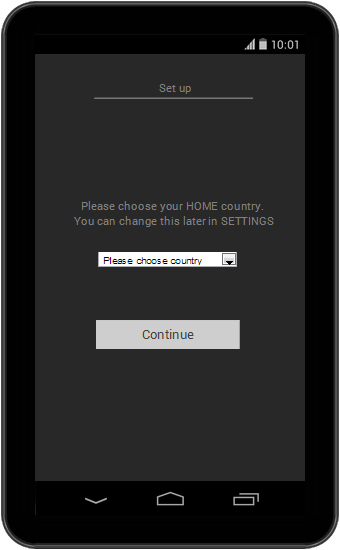
\includegraphics[scale=0.4]{mocks/setup.png}
\caption{Initial setup}
\end{figure}

\subsubsubsection{Home country overview}
This will show the main economic indicators of the user's home country. Each indicator can be tapped to open its detailed view.

The top bar is persistent throughout the application. It identifies the current view and provides options for the current view. The settings button is always in the top bar.

\begin{figure}[H]
\centering
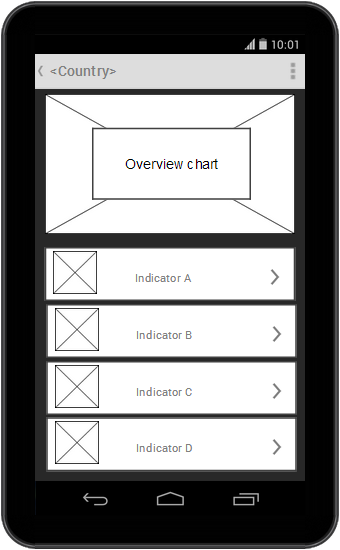
\includegraphics[scale=0.4]{mocks/overview.png}
\caption{Home country overview}
\end{figure}

\subsubsubsection{Indicator detailed view}
This will show historical information about the indicator e.g. trend of the indicator with time. If the indicator is composed of other indicators, the breakdown will also be shown in a visualisation.

Visualisations are located in a viewport at the top of the screen. Only one visualisation is shown at a time; the user can go through the visualisations by swiping the viewport (or pressing arrows on the sides of the viewport).

In this view, the top bar contains additional buttons for sharing and commenting.

\begin{figure}[H]
\centering
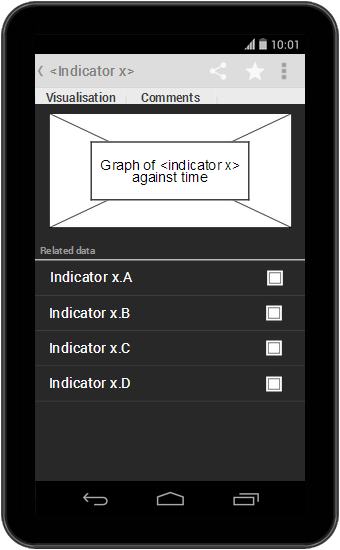
\includegraphics[scale=0.4]{mocks/detailed_single.png}
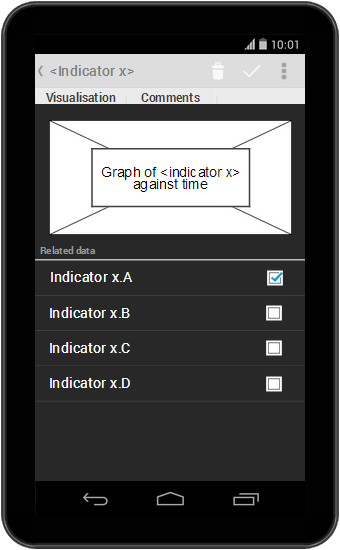
\includegraphics[scale=0.4]{mocks/detailed_single_checked.png}
\caption{Initial detailed view}
\end{figure}

\subsubsubsection{Comments view}
In this view, users can comment on a particular visualisation and read other people's comments in a comment feed. The name field will be automatically filled based on the user profile which can be configured in the application settings.

\begin{figure}[H]
\centering
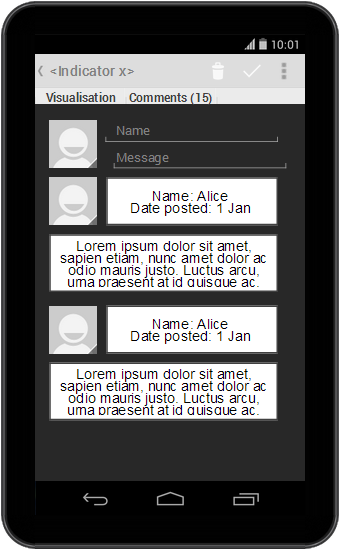
\includegraphics[scale=0.4]{mocks/comments.png}
\caption{Comments view}
\end{figure}

\subsubsubsection{Indicator comparison view}
The user can select an indicator to compare across a set of countries he/she will also choose. Upon confirmation, the appropriate visualisation will be displayed.

In this view, the top bar contains additional buttons for sharing.

\begin{figure}[H]
\centering
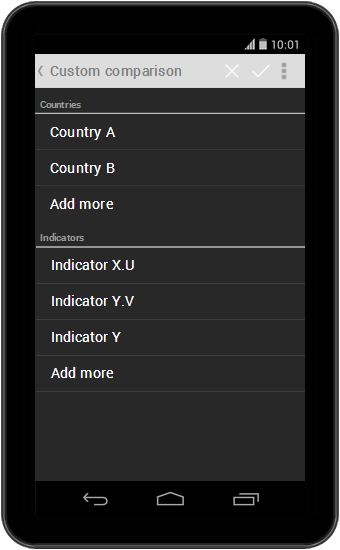
\includegraphics[scale=0.4]{mocks/compare1.png}
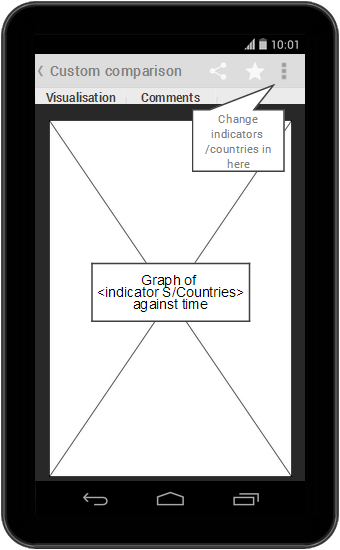
\includegraphics[scale=0.4]{mocks/compare2.png}
\caption{Indicator comparison view}
\end{figure}

\subsubsection{Hardware interfaces}
There are no explicit hardware interfaces as this is a purely software-driven application.

\subsubsection{Software interfaces}
The client-side application will run on the Cordova framework on the Android operating system (2.3 and above). The server-side components will be written in Java with a MySQL database backend.

\subsubsection{Communication interfaces}
The application will connect to the Internet via the Android operating system. Communication with the server will be via HTTP GET/POST requests.

\section{Components}

\subsection{Data retrieval component}
This server-side component will aggregate data from various sources (such as the World Bank), and store it in a database. It will also be able to check the sources for any updates to the data that it is currently storing. This component will also provide an API to the Android application to request the data. This server-side component will accept HTTP GET requests (URLs) from the Android application and return the requested data in JSON.

\subsection{Data explanation component}
This client-side component will provide explanations for indicators to allow users to better understand the indicators' significances and to better interpret the data. It will also explain how the visualisations are derived.

In an indicator detailed view, the component will explain the meaning and significance of the indicator. In an indicator comparison view, the component will explain how to interpret the visualisation.

\subsection{Data visualisation component}
This client-side component will provide a few standard visualisations to represent data. The component will take in data in JSON with visualisation parameters and return visualisations generated by a JavaScript visualisation library. The visualisations will have a unique identifier for sharing and caching purposes, and must fit nicely on the phone screen and resize accordingly if necessary.

\subsection{Comment display and input component}
This client-side component will send a HTTP GET request to the server for comments for the current indicator view and display the returned comments in a comment feed. This component will also handle user's comments and pass it on to the server.

The component must also sanitise user input to prevent any injection attacks. Comments should be limited to text only.

\subsection{Comment storage component}
This server-side component will accept HTTP POST requests containing user-submitted comments from the Android application and store them in the database backend. This server-side component will also accept HTTP GET requests for comments from the Android application and return the requested comments in JSON.

Every comment will contain the name and e-mail address of the commenter (potentially anonymous), with a reference to the view for which the comment was posted.

\subsection{Sharing component}
This client-side component will allow the user to share views in the application on the Internet. The component will generate a URL (which anybody can access with a browser) to obtain the same view as in the application. The URL is then passed into Android's sharing interface, which, depending on the user's phone, will provide a list of possible avenues for sharing. The shared view should be responsive in design and displayed appropriately in web browsers, e.g. with enlarged visualisations.

\subsection{UI and UX component}
This component ensures that our application is user friendly and conforms to the standards set out by Google's Android Developers website. It should follow design guidelines and provide a familiar user interface.

\section{Performance requirements}

\subsection{Accuracy}
Accessible economic data is useless if it is not accurate. The data in the database should not be more than one month old.

\subsection{Performance}
The application must use minimal bandwidth: only raw data should be obtained by the application, which uses its own libraries to render the visualisations. Data requests should be limited to only the following: loading overviews for the first time, loading details views of indicators for the first time, loading comparison views for the first time, and a scheduled callback to the server to check for updates to cached data. 

The interface should be fast and responsive even on low-cost phones. Visualisations should finish rendering under three seconds. This will demonstrate the feasibility of having such an application on low-cost phones and low-bandwidth Internet connections.

\section{Project management and plan}

\subsection{Roles and responsibilities}
\setlength{\extrarowheight}{5pt}
\begin{tabular}{|m{5.5cm}|m{9.5cm}|}
\hline
\textbf{Group member} & \textbf{Core Responsibilities}\\
\hline
Daniel Low &  Project manager, Visualisation, sharing \\
\hline
Darren Foong & Data retrieval, comment storage \\
\hline
Jovan Powar & Visualisations, data explanations, UI and UX\\
\hline
Samuel Haines & Data retrieval, comment storage\\
\hline
Ramankur Sen & Visualisations, data explanations, UI and UX\\
\hline
\end{tabular}

\subsection{Schedule}

\subsubsection{1 to 7 Feb 2014}
\begin{itemize}
	\item Up to \textbf{10} hours per person spent on implementing the various modules and components required. The modules can be broadly categorised into:
		\begin{itemize}
			\item Data retrieval and storage.
			\item Visualisation module for producing the visualisation based on data.
			\item Frontend UI and UX for the design and feel of the application.
			\item Application glue code to link the various components together.
		\end{itemize}
	\item The first prototype will be created.
\end{itemize}

\subsubsection{8 to 14 Feb 2014}
\begin{itemize}
	\item Up to \textbf{8} hours per person spent on testing the modules and coming up with improvements. A report on the implementation and testing will be generated.
	\item Up to \textbf{2} hours will be spent on documenting the various components' functionalities.
	\item The second prototype will be created and presented to the client on 14 Feb 2014, along with a progress report and documentation.
\end{itemize}

\subsubsection{15 to 21 Feb 2014}
\begin{itemize}
	\item Up to \textbf{6} hours spent on comments and possible modifications based on client's requirements.
	\item Up to \textbf{2} hours spent on fixing bugs found.
	\item Up to \textbf{2} hours spent on updating the documentation.
	\item The third prototype will be created.
\end{itemize}

\subsubsection{22 to 28 Feb 2014}
\begin{itemize}
	\item Up to \textbf{4} hours spent on writing group report and personal reports.
	\item Up to \textbf{4} hours spent on testing and fixing bugs.
	\item Up to \textbf{2} hours of updating documentation.
	\item The final product will be created and presented to the client on 28 Feb 2014. The group will furnish a group report, and each group member will produce a personal report.
\end{itemize}

\subsection{Prototypes}
An iterative development process is used for this project, with the aim of creating prototypes every week. We will be meeting the client on 14 and 28 Feb 2014, when we can show him a prototype personally, and solicit feedback and comments. For every prototype, we will also request for comments and feedback within the team, which we will use to develop the next iteration of the application.

\subsubsection{First prototype}
The data retrieval and data visualisation components will be implemented. The application will be able to request data from the server and render an appropriate visualisation. The server will be implemented to provide a minimal RESTful API for the application
and retrieve data from multiple data sources. The design of the application user interface will be of low priority at this stage.

\subsubsection{Second prototype}
The user interface and visualisations will be improved. The server will have the capability to parse and process data from multiple data sources and provide the processed data through a uniform RESTful API for the application's custom needs. The comment component and sharing features will be implemented. The web version of the application will be usable (for social media sharing purposes).

\subsubsection{Third prototype}
Changes proposed by client and team feedback will be considered and implemented here. Further improvements and extensive testing on the various components will be carried out.

\subsubsection{Final build}
The final prototype will meet all the abovementioned requirements, acceptance criteria, and any additional requests from the client during the development process.

\end{document}
